\documentclass[11pt,openany,oneside]{book}
\usepackage[a4paper,top=25mm,bottom=23mm,left=25mm,right=22mm,headheight=22pt]{geometry}
\usepackage{fontspec}
\setmainfont{DejaVu Serif}
\setsansfont{DejaVu Sans}
\usepackage{amssymb,xcolor,graphicx,array,booktabs,longtable,tabularx,colortbl,enumitem,tikz,tcolorbox,fancyhdr,titlesec,tocloft,hyperref,eso-pic,microtype,listings}
\usetikzlibrary{arrows.meta,positioning,shapes.geometric,calc}
\definecolor{Navy}{HTML}{17365D}
\definecolor{Teal}{HTML}{007F86}
\definecolor{Pale}{HTML}{EAF6F7}
\definecolor{Gold}{HTML}{E3A72F}
\definecolor{Ink}{HTML}{293746}
\definecolor{LightGold}{HTML}{FFF5DD}
\definecolor{SoftGray}{HTML}{F4F6F9}
\definecolor{Coral}{HTML}{D95D50}
\definecolor{Violet}{HTML}{7656A6}
\definecolor{Sky}{HTML}{DCEEFF}
\definecolor{Rose}{HTML}{FCEBE8}
\hypersetup{colorlinks=true,linkcolor=Teal,urlcolor=Teal,pdftitle={Artificial Intelligence Assistant -- Grade X},pdfauthor={Vocational Learning Textbook}}
\setlist[itemize]{leftmargin=1.5em,itemsep=1.5pt,topsep=2pt,parsep=0pt}
\setlist[enumerate]{leftmargin=1.7em,itemsep=2pt,topsep=2pt,parsep=0pt}
\setlength{\parindent}{0pt}
\setlength{\parskip}{3pt}
\setlength{\emergencystretch}{3em}
\lstdefinestyle{pythonstyle}{language=Python,basicstyle=\ttfamily\small,keywordstyle=\color{Navy}\bfseries,commentstyle=\color{Teal},stringstyle=\color{Violet},numbers=left,numberstyle=\tiny\color{Ink!65},stepnumber=1,numbersep=8pt,showstringspaces=false,breaklines=true,frame=single,rulecolor=\color{Teal!55},backgroundcolor=\color{SoftGray},xleftmargin=2mm,framexleftmargin=2mm,aboveskip=5pt,belowskip=5pt}
\AddToShipoutPictureBG{\begin{tikzpicture}[remember picture,overlay]\draw[Navy!65,line width=.55pt] ([xshift=11mm,yshift=-11mm]current page.north west) rectangle ([xshift=-11mm,yshift=11mm]current page.south east);\draw[Teal,line width=1.6pt] ([xshift=11mm,yshift=-11mm]current page.north west)--([xshift=37mm,yshift=-11mm]current page.north west);\draw[Coral,line width=1.6pt] ([xshift=-11mm,yshift=11mm]current page.south east)--([xshift=-37mm,yshift=11mm]current page.south east);\fill[Gold] ([xshift=11mm,yshift=-11mm]current page.north west) circle (1.1mm);\fill[Violet] ([xshift=-11mm,yshift=11mm]current page.south east) circle (1.1mm);\end{tikzpicture}}
\pagestyle{fancy}
\fancyhf{}
\fancyhead[L]{\raisebox{-3.5mm}[0pt][0pt]{\small\bfseries\sffamily\color{Teal} ARTIFICIAL INTELLIGENCE ASSISTANT}}
\fancyhead[R]{\raisebox{-3.5mm}[0pt][0pt]{\small\sffamily\color{Navy} GRADE X TEXTBOOK}}
\fancyfoot[C]{\tikz[baseline=(n.base)]\node[fill=Teal,draw=Gold,line width=.7pt,text=white,circle,minimum size=7mm,inner sep=1pt,font=\small\bfseries] (n) {\thepage};}
\renewcommand{\headrulewidth}{.5pt}
\renewcommand{\headrule}{\hbox to\headwidth{\color{Gold}\leaders\hrule height \headrulewidth\hfill}}
\fancypagestyle{plain}{\fancyhf{}\fancyhead[L]{\raisebox{-3.5mm}[0pt][0pt]{\small\bfseries\sffamily\color{Teal} ARTIFICIAL INTELLIGENCE ASSISTANT}}\fancyhead[R]{\raisebox{-3.5mm}[0pt][0pt]{\small\sffamily\color{Navy} GRADE X TEXTBOOK}}\fancyfoot[C]{\tikz[baseline=(n.base)]\node[fill=Teal,draw=Gold,line width=.7pt,text=white,circle,minimum size=7mm,inner sep=1pt,font=\small\bfseries] (n) {\thepage};}\renewcommand{\headrulewidth}{.5pt}\renewcommand{\headrule}{\hbox to\headwidth{\color{Gold}\leaders\hrule height \headrulewidth\hfill}}\renewcommand{\footrulewidth}{0pt}}
\titleformat{\chapter}[display]{\normalfont\sffamily\bfseries\color{Navy}}{\filleft\Large\color{Coral}\chaptername\ \thechapter}{.6ex}{\color{Teal}\LARGE\raggedright}[\vspace{.5ex}\color{Gold}\rule{\textwidth}{.8pt}]
\titlespacing*{\chapter}{0pt}{-8mm}{.5ex}
\titlespacing*{\section}{0pt}{1.2ex plus .2ex minus .2ex}{.35ex}
\titlespacing*{\subsection}{0pt}{1ex plus .2ex minus .2ex}{.3ex}
\titleformat{\section}{\Large\sffamily\bfseries\color{Teal}}{\color{Coral}\thesection}{.7em}{}
\titleformat{\subsection}{\large\sffamily\bfseries\color{Violet}}{\thesubsection}{.7em}{}
\newcommand{\exampractice}[1]{\begin{tcolorbox}[colback=LightGold,colframe=Gold,boxrule=.6pt,arc=1.2mm,left=2mm,right=2mm,top=1mm,bottom=1mm]\textbf{Review questions.} #1\end{tcolorbox}}
\newcommand{\keyterm}[1]{\textbf{\color{Navy}#1}}
\begin{document}
\begin{titlepage}\thispagestyle{empty}
\begin{tikzpicture}[remember picture,overlay]
\fill[Navy] (current page.north west) rectangle ([yshift=-11.4cm]current page.north east);
\fill[Teal] ([yshift=-11.4cm]current page.north west) rectangle ([yshift=-11.68cm]current page.north east);
\fill[Coral] ([yshift=-11.68cm]current page.north west) rectangle ([yshift=-11.82cm]current page.north east);
\draw[Gold,line width=2pt] ([xshift=22mm,yshift=-20mm]current page.north west)--([xshift=-22mm,yshift=-20mm]current page.north east);
\draw[Gold,line width=1pt] ([xshift=22mm,yshift=-103mm]current page.north west)--([xshift=-22mm,yshift=-103mm]current page.north east);
\end{tikzpicture}
\vspace*{20mm}{\color{white}\rmfamily\bfseries\fontsize{38}{44}\selectfont HANDBOOK\par}
\vspace{5mm}{\color{Gold}\rule{.72\textwidth}{1.2pt}\par}
\vspace{7mm}{\color{white}\sffamily\LARGE Artificial Intelligence Assistant\par}
\vspace{3mm}{\color{white}\sffamily\large Grade X -- Vocational Education\par}
\vfill
\begin{center}{\sffamily\Large\bfseries\color{Teal} Python \textbullet\ NumPy \textbullet\ Pandas \textbullet\ Neural Networks \textbullet\ AI Project\par}\vspace{4mm}{\sffamily\large\color{Ink} A textbook-style learning resource with examples, diagrams, code and review questions\par}\end{center}
\vfill
\begin{center}{\small Prepared with reference to the supplied Grade X study material\par}\end{center}
\end{titlepage}
\frontmatter
\tableofcontents
\mainmatter

\chapter{Python Programming}
\section{Control structures in Python}
A Python program normally executes statements in the order in which they appear. Control structures let a program choose between alternatives or repeat a set of instructions. These structures are important when a solution must respond to different inputs rather than follow one fixed path.

\subsection{Selection with \texttt{if}, \texttt{if...else} and \texttt{if...elif...else}}
An \texttt{if} statement tests a condition. If the condition is true, its indented block runs. An \texttt{if...else} statement provides an alternative when the condition is false. An \texttt{if...elif...else} ladder checks several conditions in sequence; the first true branch is executed.

\begin{lstlisting}[style=pythonstyle]
marks = int(input("Enter marks: "))
if marks >= 80:
    print("Grade A")
elif marks >= 60:
    print("Grade B")
elif marks >= 40:
    print("Grade C")
else:
    print("Needs improvement")
\end{lstlisting}
Indentation is part of Python syntax. Statements belonging to a branch must be indented consistently. Conditions can use comparison operators such as \texttt{==}, \texttt{!=}, \texttt{>}, \texttt{<}, \texttt{>=} and \texttt{<=}, along with logical operators \texttt{and}, \texttt{or} and \texttt{not}.

\subsection{Repetition using loops}
A \texttt{for} loop iterates over items in a sequence or over values produced by \texttt{range()}. A \texttt{while} loop repeats while its condition remains true. Every loop should make progress toward termination; otherwise, a \texttt{while} loop can continue indefinitely.

\begin{lstlisting}[style=pythonstyle]
total = 0
for number in range(1, 6):
    total += number
print("Total:", total)
\end{lstlisting}
The program adds the integers from 1 through 5. The \texttt{range(1, 6)} expression stops before 6, so the values are 1, 2, 3, 4 and 5. A nested loop is a loop placed inside another loop and is useful for tables, patterns and two-dimensional data.

\begin{center}
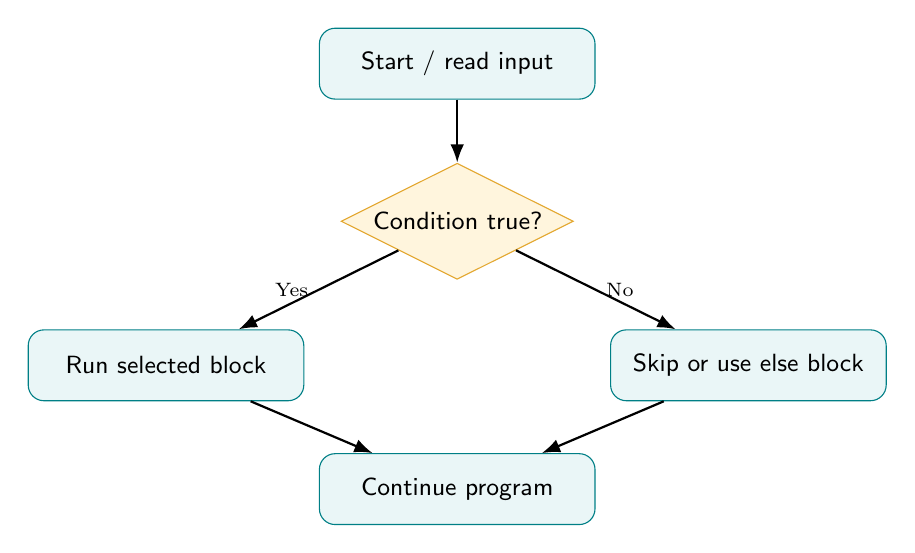
\begin{tikzpicture}[node distance=8mm,every node/.style={font=\small\sffamily,align=center},process/.style={rounded corners=2mm,draw=Teal,fill=Pale,minimum width=35mm,minimum height=9mm},decision/.style={diamond,aspect=2,draw=Gold,fill=LightGold,text width=23mm,inner sep=1pt}]
\node[process] (start) {Start / read input};
\node[decision,below=of start] (test) {Condition true?};
\node[process,below left=10mm and 12mm of test] (yes) {Run selected block};
\node[process,below right=10mm and 12mm of test] (no) {Skip or use else block};
\node[process,below=22mm of test] (end) {Continue program};
\draw[-{Latex},thick] (start)--(test);
\draw[-{Latex},thick] (test)--node[left,font=\scriptsize]{Yes}(yes);
\draw[-{Latex},thick] (test)--node[right,font=\scriptsize]{No}(no);
\draw[-{Latex},thick] (yes)--(end);
\draw[-{Latex},thick] (no)--(end);
\end{tikzpicture}
\end{center}
\textit{Figure 1.1.} A simplified decision flow for a conditional statement.

\section{Functions in Python}
A function is a named, reusable block of code that performs a task. Functions help divide a larger problem into smaller parts, reduce repetition and make a program easier to test. Python includes built-in functions such as \texttt{print()}, \texttt{len()} and \texttt{sum()}; programmers can also define their own functions with \texttt{def}.

\begin{lstlisting}[style=pythonstyle]
def mean(values):
    if len(values) == 0:
        return None
    return sum(values) / len(values)

marks = [72, 81, 67, 90]
print(mean(marks))
\end{lstlisting}
The function accepts a list as an argument and returns its arithmetic mean. The \texttt{return} statement sends a result back to the calling code. Parameters are names in a function definition; arguments are the values supplied when it is called. A local variable created inside a function is normally available only within that function.

\begin{center}
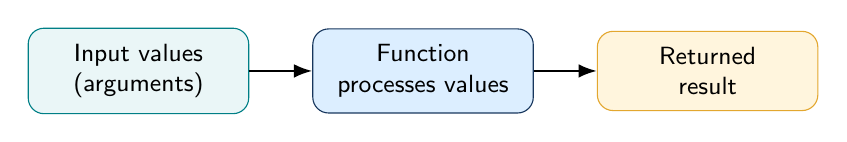
\begin{tikzpicture}[node distance=8mm,every node/.style={font=\small\sffamily,align=center},fbox/.style={rounded corners=2mm,draw=Teal,fill=Pale,minimum width=28mm,minimum height=10mm,inner sep=2mm}]
\node[fbox] (input) {Input values\\(arguments)};
\node[fbox,right=of input,draw=Navy,fill=Sky] (func) {Function\\processes values};
\node[fbox,right=of func,draw=Gold,fill=LightGold] (out) {Returned\\result};
\draw[-{Latex},thick] (input)--(func);
\draw[-{Latex},thick] (func)--(out);
\end{tikzpicture}
\end{center}
\textit{Figure 1.2.} A function receives arguments, performs a task and may return a result.

\subsection{Parameters, return values and scope}
Functions may accept zero or more parameters. A function that returns a value can be used in an expression, while a function that only performs an action may return \texttt{None}. Variables defined inside a function have local scope. Clear names, short functions and appropriate validation improve readability and reliability.

\section*{Review Questions}
\begin{enumerate}
\item Distinguish between \texttt{if...else} and \texttt{if...elif...else}.
\item What is the difference between a \texttt{for} loop and a \texttt{while} loop?
\item Write a function that returns the larger of two numbers.
\item Explain why indentation matters in Python.
\end{enumerate}

\chapter{Data Science with NumPy}
\section{Introduction to NumPy}
NumPy is a Python library for numerical computing. Its central data structure is the multidimensional array, commonly called an \texttt{ndarray}. Compared with ordinary Python lists, NumPy arrays support convenient element-wise operations and efficient numerical processing. NumPy is widely used as a foundation for scientific computing and data analysis.

\begin{lstlisting}[style=pythonstyle]
import numpy as np
marks = np.array([72, 81, 67, 90])
print(marks.mean())
print(marks.max())
print(marks.min())
\end{lstlisting}
The import statement makes NumPy available under the short name \texttt{np}, a common convention. The array stores four numerical values. Its methods calculate the mean, maximum and minimum without requiring a manually written loop.

\subsection{Array properties}
The \texttt{ndim} attribute reports the number of dimensions, \texttt{shape} reports the size along each dimension, \texttt{size} gives the total number of elements, and \texttt{dtype} indicates the element data type. A one-dimensional array can represent a sequence; a two-dimensional array can represent rows and columns.

\begin{center}
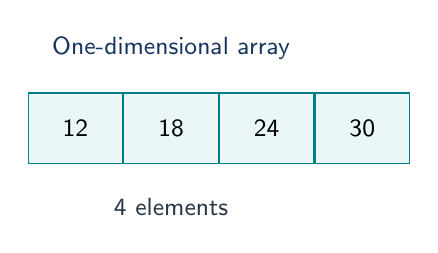
\begin{tikzpicture}[every node/.style={font=\small\sffamily},cell/.style={draw=Teal,fill=Pale,minimum width=12mm,minimum height=9mm}]
\node[cell] (a1) at (0,0) {12};
\node[cell,right=0pt of a1] (a2) {18};
\node[cell,right=0pt of a2] (a3) {24};
\node[cell,right=0pt of a3] (a4) {30};
\node[above=3mm of a2,align=center,text=Navy] {One-dimensional array};
\node[below=3mm of a2,align=center,text=Ink] {4 elements};
\end{tikzpicture}
\end{center}
\textit{Figure 2.2.} A one-dimensional NumPy array stores an ordered sequence of values.

\begin{lstlisting}[style=pythonstyle]
table = np.array([[10, 20, 30],
                  [40, 50, 60]])
print(table.ndim)   # 2
print(table.shape)  # (2, 3)
print(table.size)   # 6
\end{lstlisting}

\section{Array manipulation}
Arrays can be reshaped, joined, split, indexed and sliced. A reshape operation changes the arrangement of elements without changing their total number. Indexing selects particular elements; slicing selects a range. The requested shape must be compatible with the number of values in the array.

\begin{lstlisting}[style=pythonstyle]
values = np.array([1, 2, 3, 4, 5, 6])
matrix = values.reshape(2, 3)
print(matrix)
print(matrix[:, 1])
\end{lstlisting}
The expression \texttt{matrix[:, 1]} selects the second column. In a slice, a colon represents a range along an axis. Understanding array shape is essential when combining data from multiple sources.

\subsection{Joining, splitting and copying}
Functions such as \texttt{np.concatenate()} join arrays along a compatible axis. Splitting functions divide arrays into smaller arrays. A view can share underlying data with another array, whereas \texttt{copy()} creates independent data. Changing a shared view may therefore affect the original array.

\section{Array computation}
NumPy supports arithmetic, comparison, logical, statistical and mathematical operations. Many operations are performed element by element. Broadcasting allows arrays with compatible shapes to participate in an operation without manually copying values.

\begin{lstlisting}[style=pythonstyle]
a = np.array([1, 2, 3])
print(a * 2)       # [2 4 6]
print(a + 10)      # [11 12 13]
print(np.sqrt(a))  # square roots
\end{lstlisting}
Common statistical functions include \texttt{sum()}, \texttt{mean()}, \texttt{median()}, \texttt{min()} and \texttt{max()}. Mathematical utilities include trigonometric functions and conversions between degrees and radians. The result type depends on the operation and input types.

\begin{center}
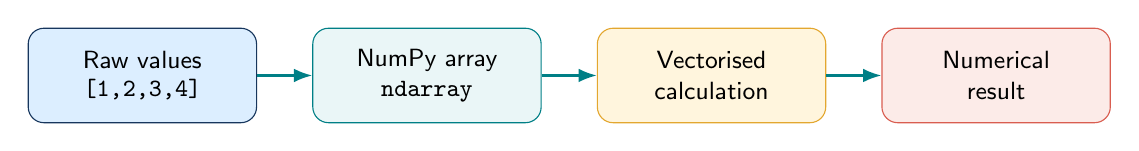
\begin{tikzpicture}[node distance=7mm,every node/.style={font=\small\sffamily,align=center},arr/.style={rounded corners=2mm,draw=Navy,fill=Sky,minimum width=29mm,minimum height=12mm}]
\node[arr] (data) {Raw values\\[-1pt]\texttt{[1,2,3,4]}};
\node[arr,right=of data,fill=Pale,draw=Teal] (array) {NumPy array\\\texttt{ndarray}};
\node[arr,right=of array,fill=LightGold,draw=Gold] (calc) {Vectorised\\calculation};
\node[arr,right=of calc,fill=Rose,draw=Coral] (result) {Numerical\\result};
\draw[-{Latex},thick,Teal] (data)--(array);
\draw[-{Latex},thick,Teal] (array)--(calc);
\draw[-{Latex},thick,Teal] (calc)--(result);
\end{tikzpicture}
\end{center}
\textit{Figure 2.1.} A typical numerical data-processing path.

\section*{Review Questions}
\begin{enumerate}
\item What do \texttt{shape}, \texttt{ndim} and \texttt{dtype} describe?
\item Explain indexing and slicing.
\item What is the difference between a view and a copy?
\item State two advantages of NumPy arrays.
\end{enumerate}

\chapter{Data Analysis}
\section{Introduction to Pandas}
Pandas is an open-source Python library used to organise, clean, analyse and summarise data. It is built around two important data structures: \texttt{Series}, a labelled one-dimensional structure, and \texttt{DataFrame}, a two-dimensional structure with rows and columns. Pandas is useful when data is arranged as a table, such as attendance records, marks, product lists or survey responses.

\begin{lstlisting}[style=pythonstyle]
import pandas as pd
students = pd.DataFrame({
    "Name": ["Asha", "Ravi", "Meena"],
    "Marks": [78, 85, 91],
    "Class": ["X", "X", "X"]
})
print(students)
print(students["Marks"].mean())
\end{lstlisting}
A DataFrame can contain columns of different data types. Column labels help identify fields, while the row index identifies records. Data should be checked for missing values, duplicate records and inconsistent formats before analysis.

\begin{center}
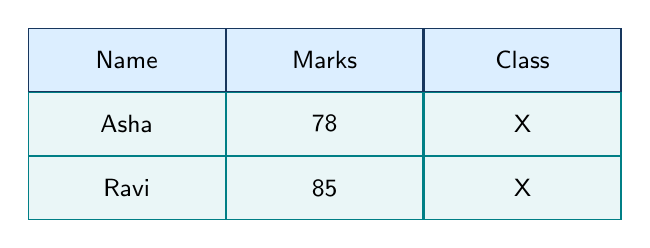
\begin{tikzpicture}[every node/.style={font=\small\sffamily,align=center},head/.style={draw=Navy,fill=Sky,minimum width=25mm,minimum height=8mm},body/.style={draw=Teal,fill=Pale,minimum width=25mm,minimum height=8mm}]
\node[head] (h1) at (0,0) {Name};
\node[head,right=0pt of h1] (h2) {Marks};
\node[head,right=0pt of h2] (h3) {Class};
\node[body,below=0pt of h1] (r11) {Asha};
\node[body,below=0pt of h2] (r12) {78};
\node[body,below=0pt of h3] (r13) {X};
\node[body,below=0pt of r11] (r21) {Ravi};
\node[body,below=0pt of r12] (r22) {85};
\node[body,below=0pt of r13] (r23) {X};
\end{tikzpicture}
\end{center}
\textit{Figure 3.2.} A simplified DataFrame with named columns and individual records.

\section{Working with Series and DataFrames}
A Series stores values with associated labels. A DataFrame groups multiple columns into a table. Pandas can create a Series from a list or dictionary, select columns, filter rows, sort values and calculate summaries.

\begin{lstlisting}[style=pythonstyle]
marks = pd.Series([72, 88, 64, 95])
print(marks.mean())
print(marks[marks >= 80])
\end{lstlisting}
Boolean filtering produces the values that satisfy a condition. In a DataFrame, a similar condition can be used to select records. Labels and positions should not be confused: label-based selection and integer-position selection have different purposes.

\subsection{Cleaning and summarising data}
Data cleaning may include handling missing values, correcting data types, removing duplicates and standardising text. The correct treatment depends on what a missing or unusual value means in the real context. Deleting records without review can distort the analysis.

\begin{lstlisting}[style=pythonstyle]
print(students.head())
print(students.info())
print(students.isna().sum())
print(students.describe())
\end{lstlisting}
The \texttt{head()} method previews records, \texttt{info()} summarises columns and data types, \texttt{isna().sum()} counts missing values by column, and \texttt{describe()} gives descriptive statistics for suitable columns.

\section{Data visualisation using Matplotlib}
Data visualisation presents information graphically so that patterns, comparisons and changes can be understood. Matplotlib is a Python library for creating charts. The chart type should match the question: bar charts compare categories, line charts show change over an ordered sequence, and scatter plots explore relationships between numerical variables.

\begin{lstlisting}[style=pythonstyle]
import matplotlib.pyplot as plt
subjects = ["English", "Maths", "Science"]
marks = [76, 88, 81]
plt.bar(subjects, marks)
plt.title("Marks by Subject")
plt.xlabel("Subject")
plt.ylabel("Marks")
plt.tight_layout()
plt.show()
\end{lstlisting}
A clear chart needs a meaningful title, labelled axes and a scale that does not mislead. Colours and decorative effects should support interpretation rather than distract from the data. Charts should be checked against the source values before conclusions are drawn.

\begin{center}
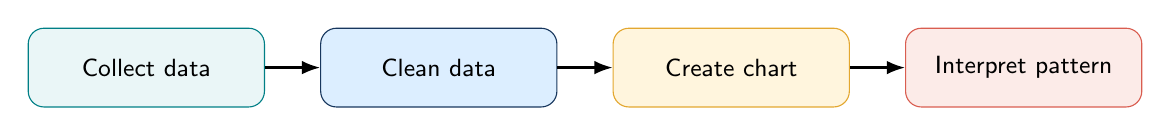
\begin{tikzpicture}[node distance=7mm,every node/.style={font=\small\sffamily,align=center},vbox/.style={rounded corners=2mm,draw=Teal,fill=Pale,minimum width=30mm,minimum height=10mm,inner sep=2mm}]
\node[vbox] (collect) {Collect data};
\node[vbox,right=of collect,draw=Navy,fill=Sky] (clean) {Clean data};
\node[vbox,right=of clean,draw=Gold,fill=LightGold] (visual) {Create chart};
\node[vbox,right=of visual,draw=Coral,fill=Rose] (interpret) {Interpret pattern};
\draw[-{Latex},thick] (collect)--(clean);
\draw[-{Latex},thick] (clean)--(visual);
\draw[-{Latex},thick] (visual)--(interpret);
\end{tikzpicture}
\end{center}
\textit{Figure 3.3.} A simple sequence for producing a trustworthy data visualisation.

\begin{center}
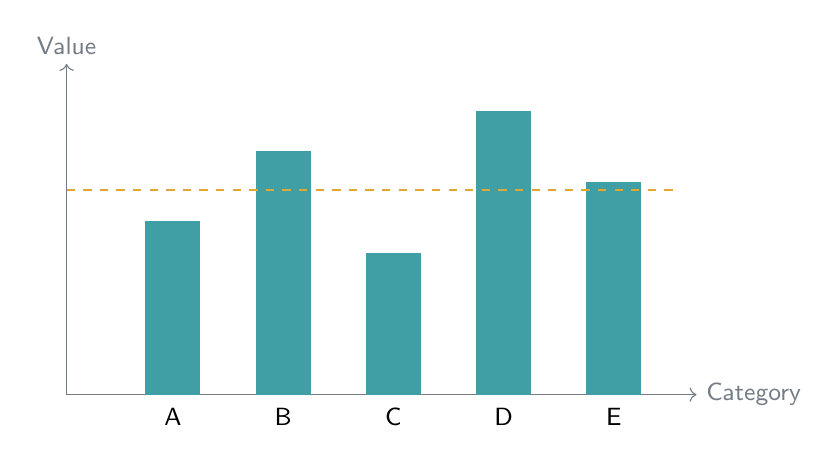
\begin{tikzpicture}[every node/.style={font=\small\sffamily}]
\draw[Ink!65,->] (0,0)--(8,0) node[right]{Category};
\draw[Ink!65,->] (0,0)--(0,4.2) node[above]{Value};
\foreach \x/\h/\lab in {1/2.2/A,2.4/3.1/B,3.8/1.8/C,5.2/3.6/D,6.6/2.7/E}{
\fill[Teal!75] (\x,0) rectangle +(0.7,\h);
\node[below] at (\x+0.35,-.05) {\lab};
}
\draw[Gold,dashed] (0,2.6)--(7.8,2.6);
\end{tikzpicture}
\end{center}
\textit{Figure 3.1.} A schematic bar chart showing how categories can be compared.

\section*{Review Questions}
\begin{enumerate}
\item Differentiate between a Series and a DataFrame.
\item Why is data cleaning necessary?
\item Name four useful Pandas methods.
\item Choose an appropriate chart to compare marks in several subjects and explain why.
\end{enumerate}

\chapter{Neural Networks and Machine Learning Tools}
\section{Artificial Neural Networks}
An Artificial Neural Network (ANN) is a computational model inspired in a broad way by networks of connected neurons. In a typical neural network, units receive numerical inputs, apply weights and a bias, pass the result through an activation function, and send outputs to the next layer. Networks can learn patterns by adjusting parameters during training.

\begin{center}
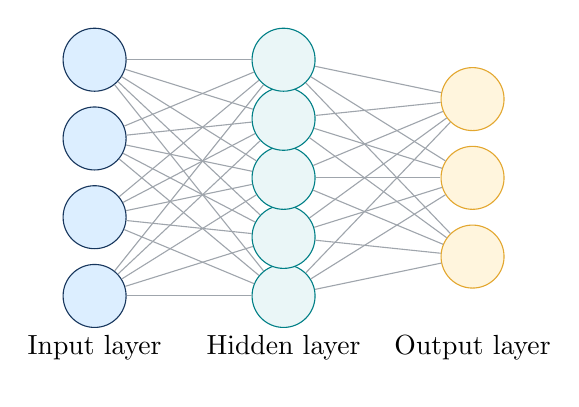
\begin{tikzpicture}[x=1cm,y=1cm,every node/.style={circle,draw=Navy,fill=Sky,minimum size=8mm,inner sep=0pt},>=Latex]
\foreach \y/\id in {0/A,1/B,2/C,3/D}{\node (i\id) at (0,\y) {};}
\foreach \y/\id in {0/A,0.75/B,1.5/C,2.25/D,3/E}{\node[fill=Pale,draw=Teal] (h\id) at (2.4,\y) {};}
\foreach \y/\id in {0.5/A,1.5/B,2.5/C}{\node[fill=LightGold,draw=Gold] (o\id) at (4.8,\y) {};}
\foreach \i in {A,B,C,D}{\foreach \h in {A,B,C,D,E}{\draw[Ink!45] (i\i)--(h\h);}}
\foreach \h in {A,B,C,D,E}{\foreach \o in {A,B,C}{\draw[Ink!45] (h\h)--(o\o);}}
\node[draw=none,fill=none,rectangle] at (0,-.65) {Input layer};
\node[draw=none,fill=none,rectangle] at (2.4,-.65) {Hidden layer};
\node[draw=none,fill=none,rectangle] at (4.8,-.65) {Output layer};
\end{tikzpicture}
\end{center}
\textit{Figure 4.1.} A simplified fully connected neural network. The drawing is conceptual; real networks can contain many layers and different connection patterns.

\subsection{Training and prediction}
During training, a network processes examples and compares its output with the expected target. A loss function measures the difference, and an optimisation method adjusts model parameters to reduce that loss. After training, the model can make predictions on new inputs. Performance on training examples alone is not enough; evaluation on separate data helps estimate how well the model generalises.

\section{Applications of neural networks}
Neural networks are used in image and speech recognition, handwriting recognition, language processing, recommendation systems, forecasting and selected healthcare applications. Face recognition can support device authentication; speech-to-text systems convert spoken language into text; recommendation systems rank items that may interest a user. Such applications can make errors, so human review and suitable safeguards remain important, especially in high-impact settings.

\subsection{Responsible use}
Data quality, privacy, fairness and transparency affect the reliability of an AI application. A model trained on unrepresentative examples may perform poorly for some groups. Sensitive personal data should be handled carefully, and a prediction should not automatically be treated as a fact. The system's purpose, limitations and evaluation results should be documented.

\section{Machine learning tools}
Python's data-science ecosystem includes tools for different stages of an AI workflow. NumPy supports numerical arrays; Pandas supports tabular data handling; Matplotlib supports visualisation; Scikit-learn provides common machine-learning algorithms and evaluation utilities; TensorFlow and Keras support the development of neural-network models; XGBoost provides optimised gradient-boosting methods.

\begin{center}
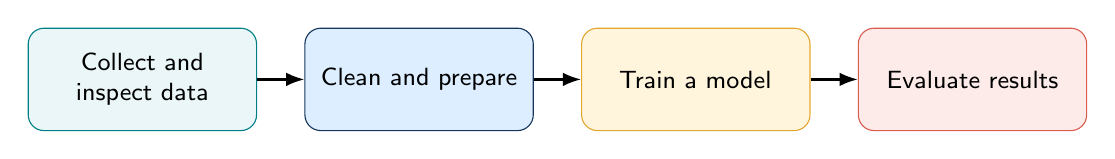
\begin{tikzpicture}[node distance=6mm,every node/.style={font=\small\sffamily,align=center},mlstage/.style={rounded corners=2mm,draw=Teal,fill=Pale,text width=25mm,minimum height=13mm,inner sep=2mm}]
\node[mlstage] (data) {Collect and inspect data};
\node[mlstage,right=of data,draw=Navy,fill=Sky] (clean) {Clean and prepare};
\node[mlstage,right=of clean,draw=Gold,fill=LightGold] (train) {Train a model};
\node[mlstage,right=of train,draw=Coral,fill=Rose] (eval) {Evaluate results};
\draw[-{Latex},thick] (data)--(clean);
\draw[-{Latex},thick] (clean)--(train);
\draw[-{Latex},thick] (train)--(eval);
\end{tikzpicture}
\end{center}
\textit{Figure 4.2.} A simplified machine-learning workflow.

\section*{Review Questions}
\begin{enumerate}
\item Name the main layers in a simple ANN.
\item What is the purpose of a loss function?
\item Give three applications of neural networks.
\item Match NumPy, Pandas, Matplotlib and Scikit-learn with their common uses.
\item Why should a model be evaluated on data not used for training?
\end{enumerate}

\chapter{AI Project}
\section{Project guidelines}
An AI project begins with a clear problem rather than with a tool. The problem statement should explain who experiences the problem, why it matters and what a useful result would look like. A manageable project has a defined scope, accessible data, a realistic schedule and criteria for evaluating the result.

\subsection{A practical project cycle}
A typical project cycle includes identifying a problem, defining the objective, collecting or selecting data, understanding and preparing the data, choosing an approach, building a prototype, testing it, evaluating outcomes and presenting findings. The stages may be revisited when testing reveals an issue.

\begin{center}
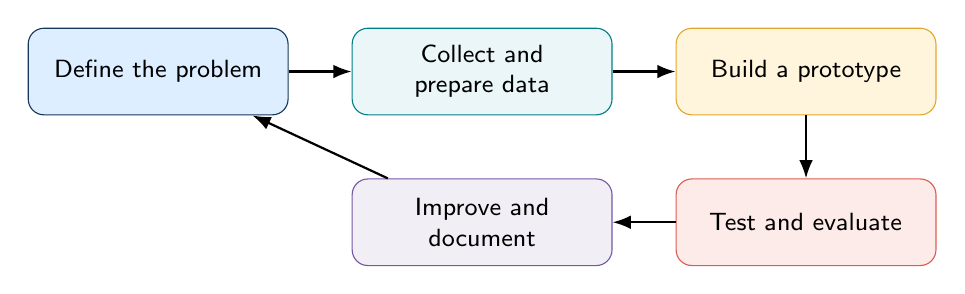
\begin{tikzpicture}[node distance=8mm,every node/.style={font=\small\sffamily,align=center},p/.style={rounded corners=2mm,draw=Navy,fill=Sky,text width=29mm,minimum height=11mm,inner sep=2mm}]
\node[p] (problem) {Define the problem};
\node[p,right=of problem,draw=Teal,fill=Pale] (data) {Collect and prepare data};
\node[p,right=of data,draw=Gold,fill=LightGold] (build) {Build a prototype};
\node[p,below=of build,draw=Coral,fill=Rose] (test) {Test and evaluate};
\node[p,left=of test,draw=Violet,fill=Violet!10] (improve) {Improve and document};
\draw[-{Latex},thick] (problem)--(data);
\draw[-{Latex},thick] (data)--(build);
\draw[-{Latex},thick] (build)--(test);
\draw[-{Latex},thick] (test)--(improve);
\draw[-{Latex},thick] (improve)--(problem);
\end{tikzpicture}
\end{center}
\textit{Figure 5.1.} An iterative project cycle. Evaluation may lead to improvements or a revised problem definition.

\section{Project formats and documentation}
A project report should communicate the problem, objective, data source, method, implementation, evaluation, limitations and conclusion. Include diagrams or tables when they make the method easier to understand. Code should be organised, named clearly and accompanied by instructions for running it. Data sources and external materials should be acknowledged.

\subsection{Choosing evaluation measures}
The measure depends on the task. A classification project may report accuracy and, where appropriate, precision, recall and a confusion matrix. A numerical prediction task may use an error measure such as mean absolute error. A visualisation project should be assessed for correctness, readability and whether it answers the original question. A single score rarely tells the whole story.

\section{Project review}
A useful review considers whether the project solves the stated problem, whether the data and method are appropriate, whether the result can be reproduced, and whether limitations are acknowledged. Reviewers should consider privacy, possible bias, safety and the consequences of incorrect predictions. Clear documentation makes the project easier to understand and maintain.

\begin{center}
\begin{tabularx}{\textwidth}{>{\bfseries}p{.25\textwidth}X}
\toprule
Review area & Questions to consider\\
\midrule
Problem and scope & Is the objective clear and achievable?\\
Data & Are the source, quality, permissions and limitations recorded?\\
Method & Is the selected approach suitable for the task?\\
Evaluation & Are the measures relevant and the results honestly reported?\\
Responsible use & Have privacy, bias and potential harm been considered?\\
Documentation & Can another person understand and reproduce the work?\\
\bottomrule
\end{tabularx}
\end{center}

\section{Sample project: student marks analysis}
A small marks-analysis project is a useful example of a data-focused AI learning task. A learner can create a table of fictional student marks, inspect the values with Pandas, calculate summaries with NumPy and present subject comparisons using Matplotlib. This project demonstrates data handling and communication; it should not be described as an AI prediction model unless a learning method is actually implemented and evaluated.

\begin{lstlisting}[style=pythonstyle]
import pandas as pd
import matplotlib.pyplot as plt

data = pd.DataFrame({
    "Subject": ["English", "Maths", "Science"],
    "Marks": [76, 88, 81]
})
print("Average:", data["Marks"].mean())
plt.bar(data["Subject"], data["Marks"])
plt.title("Sample Marks by Subject")
plt.ylabel("Marks")
plt.tight_layout()
plt.show()
\end{lstlisting}
The values are illustrative, not real student records. A report should describe the data, explain each step, include the chart, note limitations and avoid identifying real learners without a valid reason and appropriate permission.

\section*{Review Questions}
\begin{enumerate}
\item List the major stages of an AI project.
\item Why is the problem statement important?
\item What should a project report contain?
\item Explain why evaluation measures depend on the task.
\item Identify two privacy or fairness questions to consider before using data.
\end{enumerate}

\chapter*{Revision Questions}
\addcontentsline{toc}{chapter}{Revision Questions}
\section*{Python programming}
\begin{enumerate}
\item Explain selection and repetition with one Python example each.
\item Write a function that accepts a list of numbers and returns its largest value.
\item What can cause a loop to run indefinitely?
\end{enumerate}
\section*{NumPy and Pandas}
\begin{enumerate}
\item Differentiate between a NumPy array and a Python list.
\item Describe three ways to inspect a Pandas DataFrame.
\item Why must missing values be examined before they are handled?
\end{enumerate}
\section*{Visualisation and neural networks}
\begin{enumerate}
\item Select suitable chart types for category comparison and change over time.
\item Describe the role of input, hidden and output layers in a neural network.
\item Explain why a model should be evaluated on separate data.
\end{enumerate}
\section*{AI projects}
\begin{enumerate}
\item Draft a short problem statement for a simple school data project.
\item Name four items that should appear in a project report.
\item Explain two responsible-use considerations for an AI project.
\end{enumerate}

\end{document}
